\section{Zweidimensionales Punktediagramm}

Da das zweidimensionale Punktediagramm weit verbreitet ist, sind sich Betrachter an diese Darstellung gewöhnt. Oft werden die Punkte in Diagramm durch eine Linie verbunden, was den Verlauf der abgebildeten Datenwerte verdeutlicht, besonders in Medien, Börsen. 

Als erstes Beispiel hat sich darum das zweidimensionale Punktediagramm, beziehungsweise falls Linien hinzugefügt werden das Liniendiagramm besonders geeignet.

\subsection{Information-Seeking Mantra}

Als Startreferenz für die Entwicklung des interaktiven Diagrammes bietet sich die von Ben Shneiderman begründeten Prinzipien für das Design graphischen Benutzeroberflächen an, die "`\textit{Information-Seeking Mantra}"'. Die Weise, wie der Benutzer mit der Oberfläche interagiert, hat Shneiderman \cite{shneiderman} festgelegt:

\begin{itemize}
	\item Überblick ("`\textit{Overview first}"')
	\item Zoomen und Filtern ("`\textit{zoom and filter}"')
	\item Details auf Abruf ("`\textit{then details-on-demand}"')
\end{itemize}

\textbf{Überblick.} Der Benutzer verschafft sich einen Überblick über die gesamte Oberfläche des Programms.

\textbf{Zoom.} Zur besseren Betrachtung vergrössert der Benutzer die Ansicht, sodass die betreffenden Elemente grösser angezeigt werden.

\textbf{Filter.} Die Filter-Funktion ermöglicht dem Nutzer, gewisse Elemente oder Elementgruppen je nach Interesse ein- und auszublenden.

\textbf{Details auf Abruf.} Falls ein Element den Nutzer besonders interessiert, besteht die Möglichkeit, dass zusätzliche relevante Informationen zum Element angezeigt werden können.

Zusätzlich formulierte Shneiderman drei weitere Schritte:

\textbf{Zusammenhänge betrachten.} Die Zusammenhänge zwischen den verschiedenen Elementen können im Programm betrachtet werden. Diesen Schritt umzusetzen ist nur bei wenigen Benutzeroberflächen sinnvoll, zum Beispiel bei der Darstellung von Baumdiagrammen und andere Diagramme mit hierarchischen Daten.

\textbf{Verlauf.} Die Interaktionen des Benutzers mit der Programmoberfläche werden aufgezeichnet. Dadurch wird das Rückgängigmachen von Interaktionen ermöglicht.

\textbf{Extraktion.} Erlaubt die Extraktion der \textit{Query-Parametern} (wie angewandte Filter, Verlauf, Zoomstufe) und durch die Interaktion extrahierte Elementgruppen ("`\textit{subcollections}"').

In dem Diagramm werden nur die Methoden \textit{Überblick}, \textit{Zoom}, \textit{Filter} und \textit{Details auf Abruf} umgesetzt. Das Mantra wurde allgemeine für Benutzeroberflächen von Programmen beschrieben, in unserer Software, einem interaktiven Diagramm, macht die Umsetzung der Schritte \textit{Zusammenhänge betrachten}, \textit{Verlauf}, \textit{Extraktion} in Bezug auf die Funktion des Diagramms weniger Sinn:

\begin{itemize}
	\item Punktediagramme oder Liniendiagramme werden nicht dazu verwendet, Daten in Hierarchieform darzustellen.
	\item Die Interaktionen im Diagramm sind zu banal, als dass eine Rückgängig-Funktion von Nutzen wäre.
	\item Die Extraktion und der Export von Query-Parametern des Diagramms ist zwar theoretisch umzusetzen, ist jedoch von minimaler Bedeutung.
	\item Zur Extraktion von "`\textit{subcollections}"' aus einem Datensatz sollte kein interaktives Diagramm verwendet werden. Eine Datenverarbeitungsapplikation ist für diese Aufgabe angemessener, da exakte Parameter zur Extraktion bestimmt werden können.
\end{itemize}

\begin{figure}[!htbp]
	\centering
	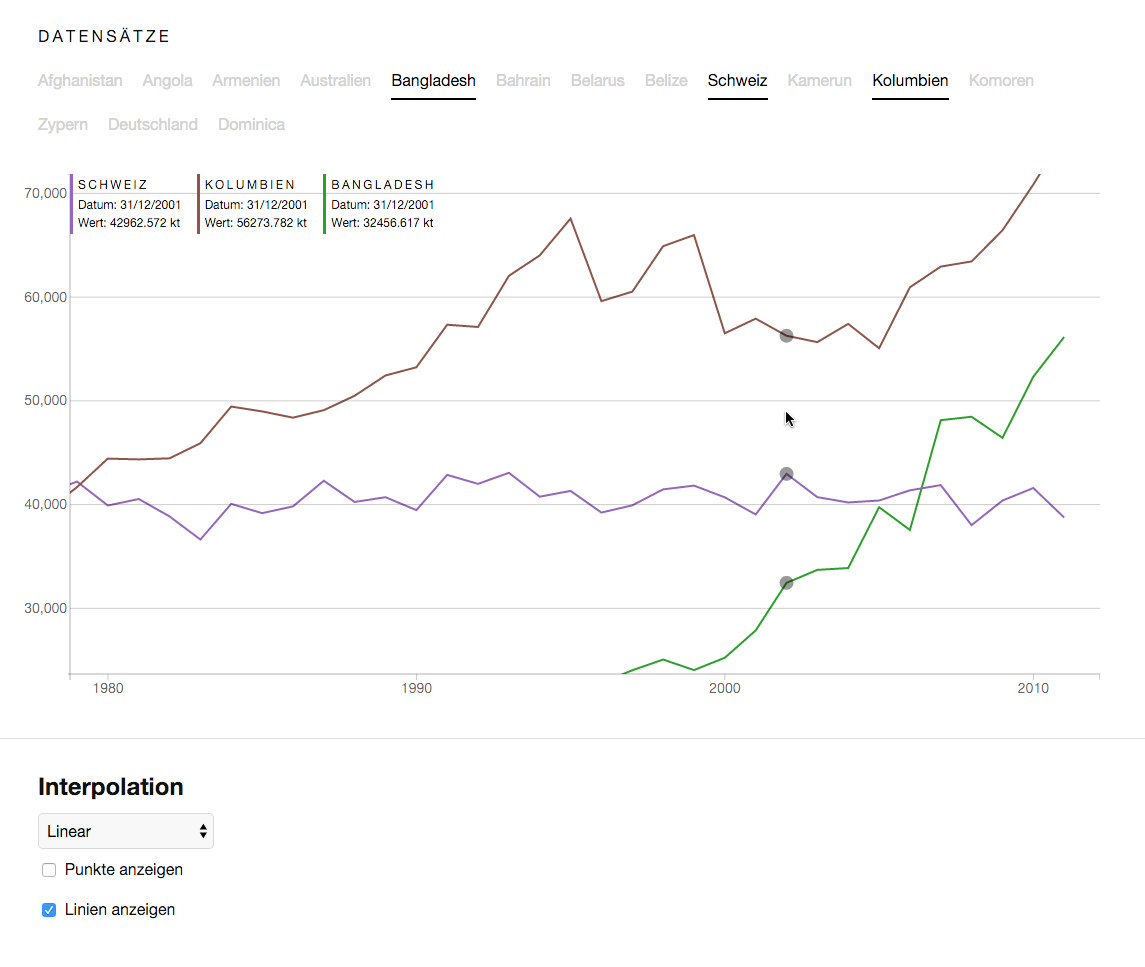
\includegraphics[width=\linewidth]{images/2dline}
	\caption[Vergleich zwischen Punktediagramm und Liniendiagramm]{Beispiel von Diagrammen am Datensatz des CO\textsubscript{2}-Verbrauchs von Afghanistan. Links: Punktediagramm. Rechts: Liniendiagramm mit linearer Interpolation.}
	\label{fig:scatterplot}
\end{figure}